\documentclass[border=6pt,tikz]{standalone}
\usepackage{tikz}
\usepackage{amsmath}
\usepackage{amssymb}
\usepackage{xcolor}
\usetikzlibrary{arrows.meta,positioning,calc,fit,backgrounds,shapes.geometric}

% --- Palette tuned to match the existing FlowchartAPUF.pdf ----------
\definecolor{blockfill}{RGB}{225,236,247}     % soft pale blue
\definecolor{blockedge}{RGB}{ 33, 64,107}     % deep navy edge
\definecolor{lanedge}  {RGB}{ 80,103,140}     % dashed lane outline
\definecolor{accent}   {RGB}{198,224,180}     % subtle green for cascade XOR
\definecolor{labelfill}{RGB}{246,249,253}

\begin{document}

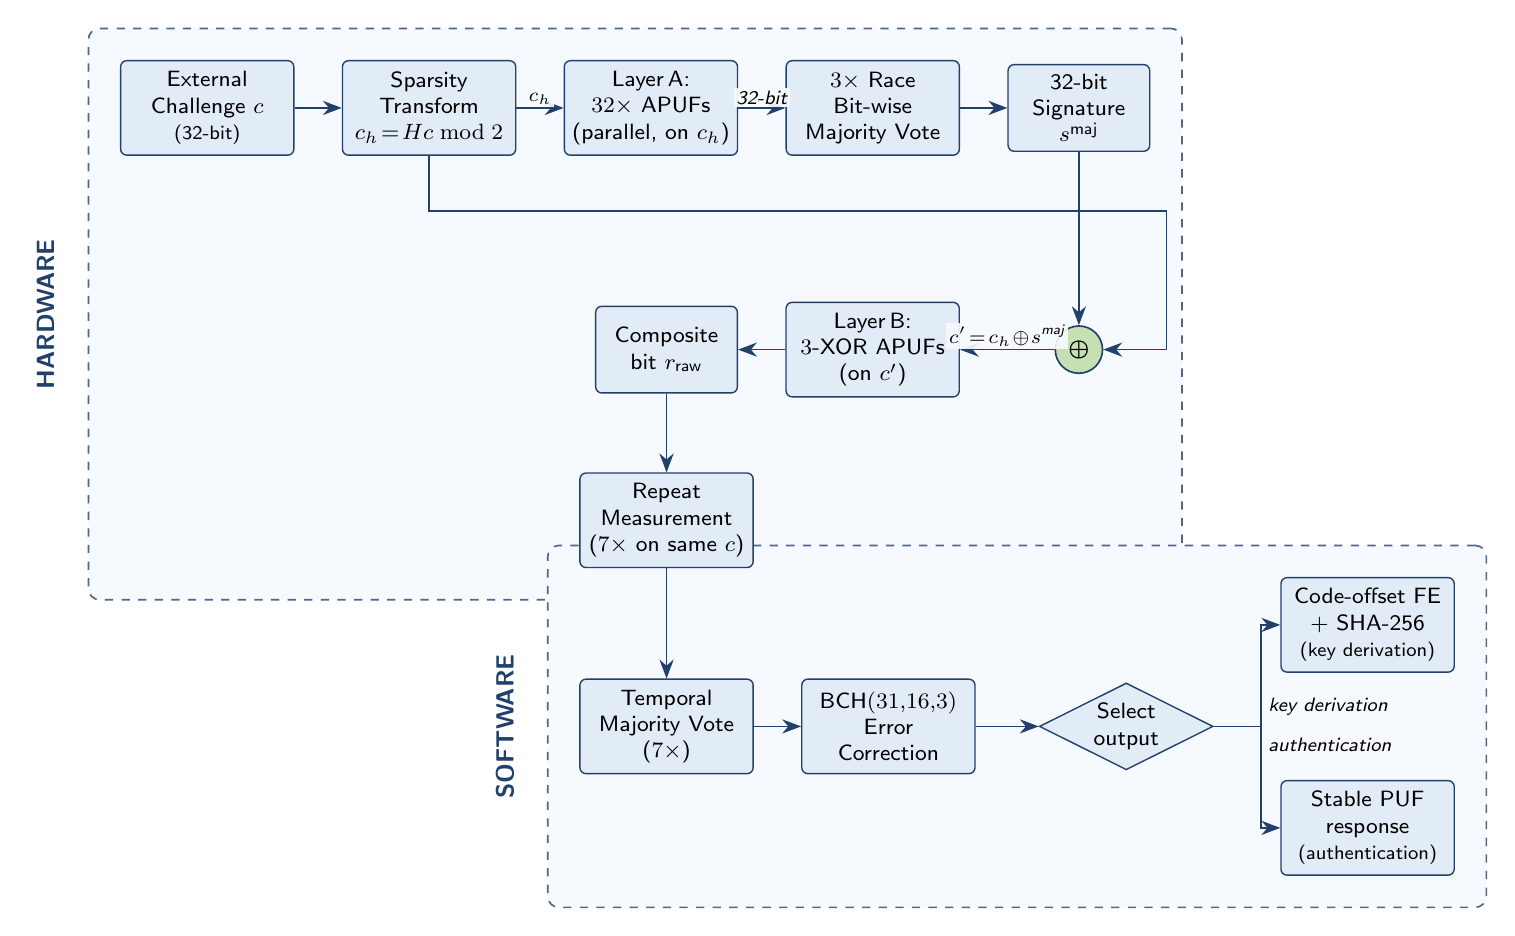
\begin{tikzpicture}[
  font=\sffamily\footnotesize,
  >={Stealth[length=2.4mm,width=1.8mm]},
  node distance=5mm and 6mm,
  every node/.style={align=center},
  block/.style={
      rectangle, rounded corners=2.2pt,
      draw=blockedge, line width=0.5pt,
      fill=blockfill,
      minimum width=22mm, minimum height=12mm,
      inner sep=2.2pt
  },
  smallblock/.style={
      rectangle, rounded corners=2.2pt,
      draw=blockedge, line width=0.5pt,
      fill=blockfill,
      minimum width=18mm, minimum height=11mm,
      inner sep=2pt
  },
  decision/.style={
      diamond, draw=blockedge, line width=0.5pt,
      fill=blockfill, aspect=2,
      inner sep=1pt, minimum width=18mm, minimum height=10mm
  },
  cascade/.style={
      circle, draw=blockedge, line width=0.6pt,
      fill=accent, inner sep=0.5pt, minimum size=6mm
  },
  arr/.style={->, draw=blockedge, line width=0.5pt},
  signal/.style={font=\sffamily\scriptsize\itshape, inner sep=1pt,
                 fill=labelfill, fill opacity=0.92, text opacity=1}
]

% =========================================================
% HARDWARE LANE -- ROW 1 (y = 0): challenge path
% =========================================================
\node[block]                          (chal)   at (0,0) {External\\Challenge $c$\\\scriptsize(32-bit)};
\node[block, right=of chal]           (htrans) {Sparsity\\Transform\\$c_h\!=\!Hc \bmod 2$};
\node[block, right=of htrans]         (layerA) {Layer\,A:\\$32{\times}$ APUFs\\(parallel, on $c_h$)};
\node[block, right=of layerA]         (rep3)   {$3{\times}$ Race\\Bit-wise\\Majority Vote};
\node[smallblock, right=of rep3]      (smaj)   {32-bit\\Signature\\$s^{\text{maj}}$};

% Row-1 arrows
\draw[arr] (chal)   -- (htrans);
\draw[arr] (htrans) -- node[signal,above]{$c_h$} (layerA);
\draw[arr] (layerA) -- node[signal,above]{32-bit} (rep3);
\draw[arr] (rep3)   -- (smaj);

% =========================================================
% HARDWARE LANE -- CASCADE + ROW 2 (y ~= -3.4)
% Layout (left-to-right): rraw, layerB, [XOR cascade] (under smaj)
% This puts XOR directly under smaj so the s_maj input is a clean
% vertical drop. The c_h tap elbows through a clear channel above
% row 2 and enters XOR from the east, with no box overlap.
% =========================================================
\node[cascade,    below=22mm of smaj]   (xor)    {\(\boldsymbol{\oplus}\)};
\node[block,      left=12mm of xor]     (layerB) {Layer\,B:\\$3$-XOR APUFs\\(on $c'$)};
\node[smallblock, left=of layerB]       (rraw)   {Composite\\bit $r_{\text{raw}}$};

% s_maj drops straight down into the cascade XOR (clean vertical)
\draw[arr] (smaj.south) -- (xor.north);

% c_h tap: from htrans.south, drop into routing channel between rows,
% travel right along the channel (which is empty), then drop into the
% east side of XOR. Channel-y is chosen above row 2 so it does not
% intersect any block.
\coordinate (chy) at ($(htrans.south)+(0,-7mm)$);            % channel y
\draw[arr] (htrans.south) -- (htrans.south |- chy)
                          -- ([xshift=8mm]xor.east |- chy)
                          -- ([xshift=8mm]xor.east)
                          -- (xor.east);

% c' output of cascade -> Layer B (with explicit equation as the label)
\draw[arr] (xor.west) -- node[signal, above]{$c'\!=\!c_h\!\oplus\!s^{\text{maj}}$} (layerB.east);
% Layer B -> r_raw (right-to-left)
\draw[arr] (layerB.west) -- (rraw.east);

% rep7 sits under rraw and transitions to the software lane
\node[block, below=10mm of rraw] (rep7) {Repeat\\Measurement\\($7{\times}$ on same $c$)};
\draw[arr] (rraw.south) -- (rep7.north);

% =========================================================
% SOFTWARE LANE -- ROW 3
% =========================================================
\node[block,    below=14mm of rep7]    (tmv)  {Temporal\\Majority Vote\\($7{\times}$)};
\node[block,    right=of tmv]          (bch)  {BCH$(31,\!16,\!3)$\\Error\\Correction};
\node[decision, right=8mm of bch]      (sel)  {Select\\output};
\node[block,    above right=4mm and 14mm of sel] (fe)   {Code-offset FE\\$+$ SHA-256\\\scriptsize(key derivation)};
\node[block,    below right=4mm and 14mm of sel] (auth) {Stable PUF\\response\\\scriptsize(authentication)};

% rep7 -> tmv
\draw[arr] (rep7.south) -- (tmv.north);
% tmv -> bch -> sel
\draw[arr] (tmv) -- (bch);
\draw[arr] (bch) -- (sel);

% Selector fan-out (two clean L-shapes, leg labels above the leg, far
% from the destination box).
\coordinate (selx) at ($(sel.east)+(6mm,0)$);
\draw[arr] (sel.east) -- (selx) |- (fe.west);
\draw[arr] (sel.east) -- (selx) |- (auth.west);
\node[signal, anchor=south west] at ($(selx)+(0.5mm,1mm)$)  {key derivation};
\node[signal, anchor=north west] at ($(selx)+(0.5mm,-1mm)$) {authentication};

% =========================================================
% Swimlane backgrounds -- drawn AFTER all nodes so the fit boxes
% capture every coordinate, but ON the background layer so they
% sit visually behind the blocks and arrows.
% =========================================================
\begin{scope}[on background layer]
  \node[draw=lanedge, dashed, line width=0.6pt, rounded corners=4pt,
        fill=labelfill, inner sep=4mm,
        fit=(chal)(htrans)(layerA)(rep3)(smaj)
            (xor)(layerB)(rraw)(rep7)]
        (hwlane) {};
  \node[draw=lanedge, dashed, line width=0.6pt, rounded corners=4pt,
        fill=labelfill, inner sep=4mm,
        fit=(tmv)(bch)(sel)(fe)(auth)]
        (swlane) {};
\end{scope}

% Lane name tags (rotated, on the left edge of each lane)
\node[anchor=south, rotate=90, font=\sffamily\bfseries\small,
      text=blockedge]
      at ([xshift=-3mm]hwlane.west) {HARDWARE};
\node[anchor=south, rotate=90, font=\sffamily\bfseries\small,
      text=blockedge]
      at ([xshift=-3mm]swlane.west) {SOFTWARE};

\end{tikzpicture}

\end{document}
